\documentclass{article}          
\usepackage{tikz}
\usetikzlibrary{positioning,shapes,fit,arrows}

\definecolor{myblue}{RGB}{56,94,141}
\begin{document}

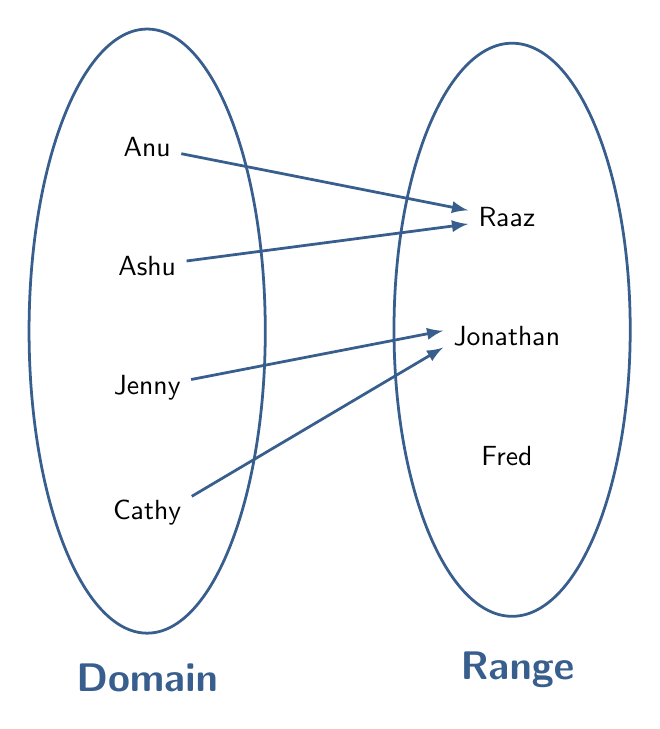
\begin{tikzpicture}[line width=1pt,>=latex]
\sffamily
\node (a1) {Anu};
\node[below=of a1] (a2) {Ashu};
\node[below=of a2] (a3) {Jenny};
\node[below=of a3] (a4) {Cathy};

\node[right=4cm of a1] (aux1) {};
\node[below= 0.5cm of aux1] (b1) {Raaz};
\node[below=of b1] (b2) {Jonathan};
\node[below=of b2] (b3) {Fred};
\node[right=4cm of a4] (aux2) {};

\node[shape=ellipse,draw=myblue,minimum size=3cm,fit={(a1) (a4)}] {};
\node[shape=ellipse,draw=myblue,minimum size=3cm,fit={(aux1) (aux2)}] {};

\node[below=1.5cm of a4,font=\color{myblue}\Large\bfseries] {Domain};
\node[below=1.5cm of aux2,font=\color{myblue}\Large\bfseries] {Range};

\draw[->,myblue] (a1) -- (b1.170);
\draw[->,myblue] (a2) -- (b1.190);
\draw[->,myblue] (a3) -- (b2.175);
\draw[->,myblue] (a4.20) -- (b2.190);
\end{tikzpicture}

\end{document}
